\section{Brownian motion}
	\label{sec:chapter1}
	
\subsection{The Brownian motion discovery}

	
In 1827 the Scottish botanist Robert Brown published a paper \cite{robert_xxvii_1828} on his observation on the pollen of \textit{Clarkia pulchella} with a lot of details on his taught processes. His experiments was made to understand the flower reproduction, but, as he was looking through the microscope he observed some minute particles ejected from the pollen grains. At first, he thought this movement was a test to of the male organ, then looking at grains Mosses and \textit{Equiseta} which had been dried up for one hundred years, he was surprised to see this "peculiar" movement and since he was able to increase the number of particle by bruising ovula or seeds of \textit{Equisetum} he abandoned his supposition. Interestingly each time that he encountered a material that he was able to reduce to a fine enough powder to be suspended in water, he observed a constant motion, although, he never guessed the origin of the particles movement.

The difficulty at this time to observe and capture this movement made the study of what we called today Brownian motion quite difficult and the first work on erratic movement was actually done by Louis Bachelier  in 1900 in his PhD thesis "The theory of speculation", where he describe a stochastic analysis of the stock and option market. The mathematical description is still a used in the modern development of tools for the economic industry. 

It's finally in 1905 that Albert Einstein describe that "bodies of microscopically visible size suspended in a liquid will perform movements of such a magnitude that they can be easily observed in a microscope". \cite{einstein_uber_1905}. A nice remark to make here is that in 1948 Einstein wrote a letter to one of his friend where he stated having deduced the Brownian motion "from mechanics, without knowing that anyone had already observed anything of the kind" \cite{peter_brownian_nodate}.

It's in 1908 that Jean Perrin published his experimental work on the Brownian motion, that way he was able to measure the Avogadro number and prove the kinetic theory that Einstein developed. I would also cite M. Chaudesaigues and M. Dabrowski, who helped J. Perrin to track the particles by hand, half-minutes by half-minutes, for more than 3000 displacements (25 hours) and several particles. This impressive and daunting work is highly detailed in "Mouvement brownien et molécules" \cite{perrin_mouvement_1910}. This is partly due to this work than J. Perrin received the nobel award in 1926.

\begin{figure}[h]
	\centering
	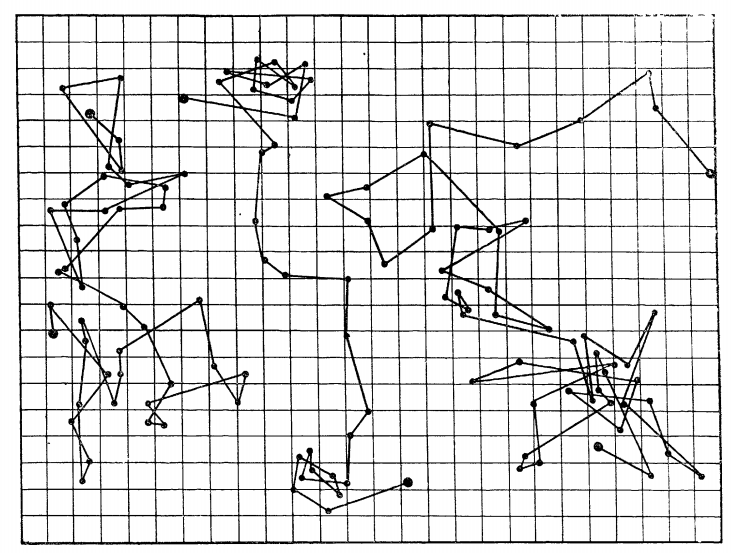
\includegraphics[scale=0.6]{02_body/chapter1/image/graph_perrin.png}
	\caption{Brownian motion of $1 ~ \mathrm{\mu m}$ particle in water tracked by hand by Jean Perrin and his colleagues, each point are timely space by 30 seconds and 16 divisions represents $50 ~ \mathrm{\mu m}$  the mean square value of was the first prove of the Einstein's kinetic theory}
	\label{fig:Perrin_Brownian}
\end{figure}

\subsection{The Einstein Brownian theory}

In this section we will derive the main characteristic of the bulk Brownian motion in the manner of Einstein in 1905 by summarizing the section 4 of \cite{einstein_uber_1905}. We will then examine  the random motion of particles suspended in a liquid and their relation to diffusion, caused bu thermal molecular motion. We assume that each particle motion is independent of other particles; also. the motion of one particle at different time interval as to to be taken independent process as long as the time interval is not too small. We know introduce a time interval $\tau$ which as to be small compered to the observation time but small enough so that  the displacement between two consecutive time intervals $\tau$ may be taken as independent events (ie. the over damped regime). 

For simplicity, we will here look only at the Brownian motion of $n$ particles in 1D along the $x$ axis. In a time interval $\tau$ the position of each individual particle will increase by a displacement $\Delta$, positive or negative and different for all the particles. The number of particle $dn$ experiencing a displacement lying between $\Delta$ and $\Delta + d\Delta$ in a time interval $\tau$ is written as:

\begin{equation}
	dn = n\varphi(\Delta)d\Delta,
\end{equation}

where

\begin{equation}
	\int_{-\infty} ^{\infty} \varphi (\Delta)d \Delta = 1,
	\label{Eq:ein_def_phi}
\end{equation}

and $\varphi$ is nonzero only for very small displacement $\Delta$ and satifies $\varphi (\Delta) = \varphi (-\Delta)$.

Let $f(x,t)$ be the number of particles per unit volume. From the definition of the function $\varphi(\Delta)$ we can obtain the distribution of particles found at time $ t + \tau$ from their distribution at a time $t$, we obtain:

\begin{equation}
	f(x, t+\tau)dx = dx\int_{\Delta = -\infty} ^{\Delta = +\infty} f(x+\Delta, t) \varphi (\Delta) d\Delta
	\label{Eq:Ein_first}
\end{equation}

Since $\tau$ is very small, we have:

\begin{equation}
	f(x, t+\tau) = f(x,t) + \tau \frac{\partial f}{\partial t}
\end{equation}

On the other side we can Taylor expend $f(x+\Delta, t)$ in powers of $\Delta$ since only small values of $\Delta$ contribute. We obtain:

\begin{equation}
	f(x + \Delta, t) = f(x,t) + \Delta \frac{\partial f(x,t)}{\partial x} + \frac{\Delta ^2}{2!} \frac{\partial ^2 f(x,t)}{\partial x^2}...
\end{equation}

Putting all together, in Eq.\ref{Eq:Ein_first} we obtain:

\begin{equation}
	f + \frac{\partial f}{\partial t} \tau = f \int_{-\infty}^{+\infty} \varphi(\Delta)d \Delta + \frac{\partial f}{\partial x} \int_{-\infty}^{+\infty} \Delta \varphi (\Delta)d \Delta + \frac{\partial ^2 f}{\partial x^2} \int_{-\infty}^{+\infty} \frac{\Delta ^2}{2} \varphi(\Delta)d\Delta ...
	\label{Eq:ein_expended}
\end{equation}

On the right-hand side, since $\varphi(x) = \varphi(-x)$ all even terms will vanish and all the odd terms will be very small compared to the precedent. If we take into account \ref{Eq:ein_def_phi} and only the first and third term of the right hand side, by putting:

\begin{equation}
	\frac{1}{\tau} \int_{-\infty}^{+\infty} \frac{\Delta^2}{2}\varphi(\Delta)d\Delta =D,
\end{equation}

the Eq.\ref{Eq:ein_expended} finally becomes:

\begin{equation}
	\frac{\partial f}{\partial t} = D \frac{\partial ^2 f}{\partial x ^2}.
\end{equation}

We can here recognize a differential equation for the diffusion with $D$ the diffusion coefficient. We will now initiate the same position $x=0$ for all the particle at $t=0$ as in the Fig. and $f(x,t)dx$ now denoting the number of particles whose position as increased between the times  $t=0$ and $t=t$  by a quantity lying between $x$ and $x + dx$ such that we must have:

\begin{equation}
	f(x \ne 0, t=0) = 0 \text{ and } \int_{-\infty}^{+\infty}f(x,t)dx = n.
\end{equation}

The solution of this equation is known and the same as the heat equation and is given by the Gaussian:


\begin{equation}
	f(x,t) = \frac{1}{\sqrt{4\pi D}} \frac{\mathrm{exp}^{\frac{-x^2}{4Dt}}}{\sqrt{t}}
\end{equation}

From this solution we can see that the mean value of the displacement of all the particles along the $x$ axis is equal to $0$ and the square root of the arithmetic mean of the squares of displacements (that we commonly call Mean Square displacement (\gls{MSD}))  is given by:
\begin{equation}
	\lambda _x = \sqrt{2Dt}
	\label{Eq:MSD_ein}
\end{equation}

The mean displacement is thus proportional to the square root of time, this result is generally the first behavior that we check when we study for the first time experimental Brownian motion. We can further suppose that in 3D, the square root of the \gls{MSD} will be given by $\lambda_x \sqrt{3}$

Previously in his paper, in the chapter 3, he had found by writing the thermodynamic equilibrium of a suspension of particles that the diffusion coefficient of a particle should be written:

\begin{equation}
	D = \frac{R T}{N_A}\frac{1}{6\pi \eta a}
	\label{Eq:D_einstein}
\end{equation}

with $R$ the gas constant, $T$ the temperature, $N_A$ the Avogadro number and $\eta$ the fluid viscosity. Thus an experimental observation measurement could lead to a measurement of the Avogadro number and the true size of the atoms since:

\begin{equation}
	N_A = \frac{t}{\lambda_x^2} \frac{RT}{3\pi \eta a}
\end{equation}

Finally he ends up is paper \cite{einstein_uber_1905} by saying \textit{"Let us hope that a researcher will soon succeed in solving the problem posed here, which is of such importance in the theory of heat!"}. I'd like here to emphasize on the importance of solving this problem in very beginning of th 19's. At this time two theory about the fundamental component existed, ones seeing only energy and a second one especially supported by Boltzmann and his kinetic theory of gases, here used by Einstein. Thus, an experimental proof of Eq.\ref{Eq:D_einstein} would prove the existence of atoms and molecules. Due to a lot of theoretical misunderstanding of the theory and experimental error scientist such as Svedberg or Henri thought that Eintein's theory was false \cite{genthon_concept_2020} by even proving that the statistical properties of the Brownian motion was changing with the pH of the solution. It's finally in 1908 that Chaudesaigues and Perrin published all the evidence to prove Einstein's theory mainly by their ability to create particle emulsion of well controlled radius. 

\begin{figure}
	\centering
	\includegraphics{02_body/chapter1/image/brown_exemple.pdf}
	\caption{Simulation of bulk Brownian motion of $1 ~ \mathrm{\mu m}$ particles in water. On the top each line represents the trajectory of a Brownian particle over 100 seconds a total of 100 trajectories or shown. On the bottom, bullets represents the \gls{MSD} computed from the simulated trajectories. The black plain line represents the Einstein's theory, which is computed from the square of Eq.\ref{Eq:MSD_ein}}.
\end{figure}